\mychapter{state-of-the-art}{State of the Art in Provisioning}

There already exists scientific research projects, APIs, frameworks 
and other technologies which aim at consolidating, interfacing and utilizing cloud technologies.
This chapter introduces some of these concepts.
First scientific research projects will be presented with their solutions, 
then pure technological approaches will be introduced.

\section{Model-Driven Approaches}

The following technologies are in some way model based.
That means they either use concrete diagrams or any other means of
modeling that can relate to Model-Driven Engineering.

\paragraph{Amazon AWS CloudFormation}~\cite{aws}

\begin{figure}[tb]
  \begin{center}
    \begin{minted}[mathescape,
                   linenos,
                   numbersep=5pt,
                   frame=lines,
                   framesep=2mm]{json}
{
  "Description": "Create an EC2 instance",
  "Parameters": {
    "KeyPair": {
      "Description": "For SSH access",
      "Type": "String"
    }
  },
  "Resources": {
    "Ec2Instance": {
      "Type": "AWS::EC2::Instance",
      "Properties": {
        "KeyName": { "Ref": "KeyPair" },
        "ImageId": "ami-1234abcd" 
      }
    }
  },
  "Outputs" : {
    "InstanceId": {
     "Description": "Instace ID of created instance",
     "Value": { "Ref": "Ec2Instance" }
    }
  },
  "AWSTemplateFormatVersion": "2010-09-09"
}
    \end{minted}
  \end{center}
  \caption{AWS CloudFormation template.}
  \label{fig:cloudformation-template}
\end{figure}



This is a service provided by Amazon from their popular \emph{Amazon Web Services}~(AWS).
It give users the ability to create template files in form of 
\emph{JavaScript Object Notation}~(JSON) as seen in ~\citefig{cloudformation-template}, 
which they can load into AWS to create stacks of resources. 
A \emph{stack} is a defined set of resources in different amount and sizes, such as numerous instances,
one or more databases and a load balancer, although what types and sizes of resources is ambiguous.
To provision a stack with CloudFormation the template file (in JSON format) is first uploaded to
AWS which makes it accessible from AWS Management Console.

The template consist of three main sections, 
\begin{ii}\iitem \emph{Parameters}, \iitem \emph{Resources} and \iitem \emph{Outputs}.\end{ii}
The \emph{Parameters} section makes it possible to send parameters into the template, 
with this the template becomes a macro language by replacing references in the \emph{Resources} section 
with inputs from users. Input to the parameters are given inside the management console when 
provisioning a stack with a given template.
The \emph{Resource} section define types of resources that should be provisioned, the \emph{Type}
property is based on a set of predefined resource types such as \emph{AWS::EC2::Instance}
in Java package style.
The last section, \emph{Output}, will generate output to users when provisioning is complete,
here it is possible for users to pick from a set of variables to get the information they need.

This template system makes it easier for users to duplicate a setup many times, 
and as the templates support parameters this process can be as dynamic as the user design it to be. 
This is a model in form or lexical syntax, both the template itself and the resources that can be used.
For a company that is fresh in the world of cloud computing this service could be considered too advance. 
This is mainly meant for users that want to replicate a certain stack, with the ability to provide custom parameters. 
Once a stack is deployed it is only maintainable through the AWS Management Console, and not through template files. 
The format that Amazon uses for the templates is a good format, the syntax is in form of JSON which is readable and easy to use, 
but the structure and semantics of the template itself is not used by any other providers or cloud management tooling, 
so it can not be considered a multicloud solution. Even though JSON is a readable format, does not make it viable as a presentation medium on a business level.

\paragraph{CA Applogic}~\cite{applogic}

\begin{figure}
  \begin{center}
  \end{center}
  \caption{CA Applogic}
    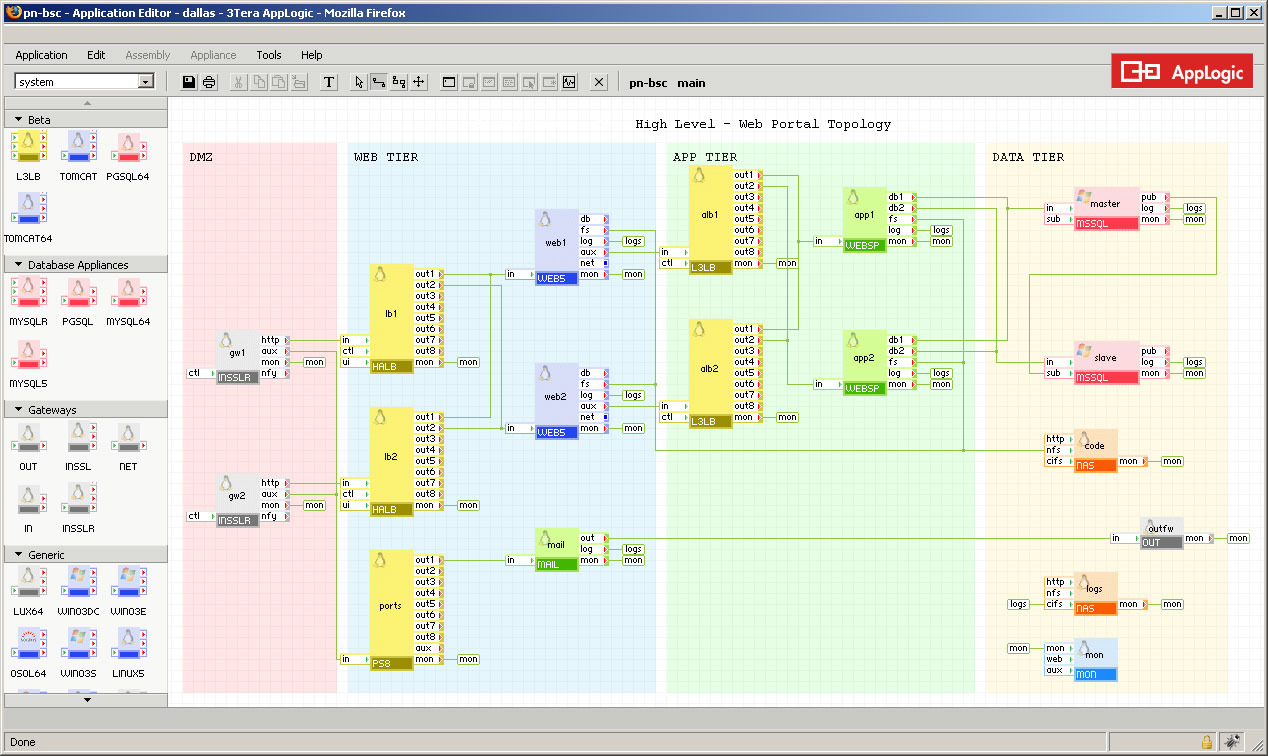
\includegraphics[width=\linewidth]{img/applogic.jpg}
  \label{fig:applogic}
\end{figure}


The Applogic platform is designed to manage CAs private cloud infrastructure~\cite{introducing-cloud-services}.
It also has a web based interface which let users manage their cloud resources 
as shown in~\citefig{applogic} which use and benefit from a model based approach.
It is based on graphical models which support interactive ``drag and drop'' functionalities.
This interface let users configure their deployments through a diagram with familiarities to 
UML component diagrams with interfaces and assembly connectors. 
They let users configure a selection of third party applications, 
such as Apache and MySQL, as well as network security, instances and monitoring. 
What CA has created is both an easy way into the cloud and it utilizes the advantages of model realizations. 
Their solution will also prove beneficial when conducting business level consulting
as it visualizes the structural layout of an application.
But this solution is only made for private clouds running their own controller, 
this can prove troublesome for migration, both in to and out of the infrastructure.

\section{APIs}

Extensive work have been done towards simplifying and combining cloud technologies through
abstractions, interfaces and integrations.
Much of this work is in form of APIs, mostly in two different forms.
Either as programming libraries that can be utilized directly from a given 
programming language or environment such as Java or Python.
The other common solution is to have an online facade against public providers,
in this solution the APIs are mostly in RESTful form.

\subparagraph{Driver.}

Many of the API solutions use the term ``\emph{driver}'', it represents
a module or component that fit into existing software and extend the support
of external connections without changing the interface.
A cloud \emph{driver} connects a given software to an existing cloud provider
through this providers web based API (REST).

\paragraph{libcloud and jclouds}~\cite{libcloud, jclouds}

Libcloud is an API that aims to support the largest cloud providers through a common API. 
The classes are based around \emph{drivers} that extends from a common ontology, then provider-specific attributes and logic is added to the implementation.
jclouds is very similar to libcloud but the API code base is written in Java and Clojure. 
This library also have \emph{drivers} for different providers, but they also support some PaaS solutions such as Google App Engine.
APIs can be considered modelling approaches based on the fact they have a topology and hierarchical structure, 
but it is not a distinct modelling. A modelling language could overlay the code and help providing a clear overview, 
but the language directly would not provide a good overview of deployment. 
And links between resources can be hard to see, as the API lacks correlation between resources and method calls. 
Libcloud have solved the multicloud problem in a very detailed manner, but the complexity is therefore even larger. 
The API is also Python-only and could therefor be considered to have high tool-chain dependency.

\paragraph{OPA}~\cite{opa}

OPA is a cloud language aimed at easing development of modern web applications. It is a new language, 
with its own syntax, which is aimed directly at the web. The language will build into executable files that will handle load balancing and scalability, 
this is to to make this a part of the language and compilation.
OPA is a new language, so it might be difficult to migrate legacy systems into this lanugage. 
There are no deployment configurations, as this is built into the language. The compiler will generate an executable that coWeb-based vs native application

In public cloud enviromants managing, monitoring, payment and other administrative 
tasks can be done through web interfaces or APIs. 
Web applications are becoming more popular by the day, with HTML5, EcmaScript 5 and CSS3. 
The user experience in web applications today can in many cases match native applications, with additional benefits such as availability and ease of use.
A web-based interface would prove beneficial for quickly displaying the simple core functionality of the language. 
In this era of cloud computing and cloud technologies a user should not need to abandon his or hers browser to explore the functionality of CloudML.
Cloud providers are most likely to give customers access to customize their cloud services through web-based interfaces, 
and if customers are to take advantage of CloudML, the language should be graphically integrated into existing tool chains. 
Providers would probably find it pleasing if a example GUI wauld be run on most cloud providers instances, 
and so it can also benefit from some cloud based load balancers, even though this is part of the language. 
The conclusion about OPA is that it is not a language meant for configuration, and could not easily benefit from a model based approach, 
and it does not intentionally solve multicloud.

\paragraph{Whirr}~\cite{whirr}

\todo{Fill this one out}

This is a binary and code-based application for creating and starting short-lived clusters for hadoop instances.
It support multiple cloud providers. It has a layout for configuration but it is mainly property-based, and aimed at making clusters. 

\paragraph{Deltacloud}~\cite{deltacloud}

Deltacloud has a similar procedure as jclouds and libcloud, but with a REST API. 
So they also work on the term \emph{driver}, but instead of having a library to a programming language the users are presented with an API they can call, 
on Deltacloud servers. This means users can write in any language they may choose. 
As well as having similar problems as other APIs this approach means that every call has to go through their servers, 
similar to a proxy. This can work with the benefits that many middleware software have, such as cahing, queues, 
redundancy and transformations, but it also has the disadvantages such as single point of failure and version inconsistencies.

\section{Deployment frameworks}

\paragraph{Amazon Beanstalk}
\paragraph{simplifying-solution-deployment-on-a-cloud-through-composite-appliances}
\paragraph{architecture-for-virtual-solution-composition-and-deployment}

\paragraph{mOSAIC}

mOSAIC~\cite{portable:petcu12} aims at not only provisioning in the cloud, but deployment as well.
They focus on abstractions for application developers and state they can easily enable users to
\emph{``obtain the desired application characteristics (like
scalability, fault-tolerance, QoS, \etc.)''}~\cite{architecturing:petcu11}.
The strongest similarities to CloudML are 
\begin{ii}\iitem multicloud with their API~\cite{architecturing:petcu11},
\iitem metadata dependencies since they support full deployment and
\iitem robustness through fault-tolerance.
What mOSAIC is lacking compared to CloudML is model-based approach including \emph{M@RT}.

\paragraph{reservoir}

Reservoir~\cite{reservoir:rochweger09} is another project that also aim at
\iitem multicloud. The other goals of this project is to leverage 
scalability in single providers and support built-in \emph{Business Service Management}~(BSM),
important topics but not directly related to the goals of CloudML.
CloudML stands out from Reservoir in the same way as mOSAIC.

\paragraph{Vega}
Vega framework~\cite{simplifying:chieu10} is a deployment framework aiming 
at full cloud deployments of multi-tier topologies, they also follow a \iitem model-based 
approach\end{ii}. The main difference between CloudML and Vega are support of multicloud provisioning.


